\chapter{Метасистема OSTIS}
\chapauthortoc{Голенков В.В.\\Шункевич Д.В.\\Банцевич К.А.\\Загорский А.Г.}
\label{chapter_ims_standard}

\vspace{-7\baselineskip}

\begin{SCn}
	\begin{scnrelfromlist}{авторы}
		\scnitem{Голенков В.В.}
		\scnitem{Шункевич Д.В.}
		\scnitem{Банцевич К.А.}
		\scnitem{Загорский А.Г}
	\end{scnrelfromlist}
		
	\bigskip
	
	\scntext{аннотация}{Данная глава посвящена рассмотрению подхода к автоматизации процессов создания, развития и применения стандартов на основе Технологии OSTIS. Также в главе сформулированы основные принципы стандартизации интеллектуальных компьютерных систем, методов и средств их проектирования в рамках предлагаемого подхода.}
	
	\bigskip
	
	\begin{scnrelfromlist}{подраздел}
		\scnitem{\ref{sec_metasystem}~\nameref{sec_metasystem}}
		\scnitem{\ref{sec_standard}~\nameref{sec_standard}}
	\end{scnrelfromlist}
	
	\bigskip
	
	\begin{scnrelfromlist}{ключевое понятие}
		\scnitem{Метасистема OSTIS}
		\scnitem{Стандарт Технологии OSTIS}
	\end{scnrelfromlist}
	
	\bigskip
	
	\begin{scnrelfromlist}{библиографическая ссылка}
		\scnitem{...}
	\end{scnrelfromlist}
	
\end{SCn}

\section*{Введение в Главу \ref{chapter_ims_standard}}

В основе каждой развитой сферы человеческой деятельности лежит ряд стандартов, формально описывающих различные ее аспекты -- систему понятий (включая терминологию), типологию и последовательность действий, выполняемых в процессе применения соответствующих методов и средств.

Стандарты в самых различных областях являются важнейшим видом знаний, главной целью которых является обеспечение совместимости различных видов деятельности.  Несмотря на развитие информационных технологий, в настоящее время подавляющее большинство стандартов представлено либо в виде традиционных линейных документов, либо в виде web-ресурсов содержащих набор статических страниц, связанных гиперссылками. Для того чтобы стандарты выполняли свою главную функцию, они должны постоянно совершенствоваться. 

Текущее оформление стандартов имеет ряд недостатков, которые мешают эффективному и грамотному использованию стандартов в различных областях:
\begin{textitemize}
	\item дублирование информации в рамках документа, описывающего стандарт;
	\item трудоемкость сопровождения самого стандарта, обусловленная в том числе дублированием информации, в частности, трудоемкость изменения терминологии;
	\item проблема интернационализации стандарта -- фактически перевод стандарта на несколько языков приводит к необходимости поддержки и согласования независимых версий стандарта на разных языках;
	\item неудобство применения стандарта, в частности, трудоемкость поиска необходимой информации. 	Как следствие – трудоемкость изучения стандарта;
	\item несогласованность формы различных стандартов между собой, как следствие – трудоемкость автоматизации процессов развития и применения стандартов;
	\item трудоемкость автоматизации проверки соответствия объектов или процессов требования того
	или иного стандарта;
	\item  и другие.
\end{textitemize}

Перечисленные проблемы связаны в основном с формой представления стандартов. 

Задачей любого стандарта в общем случае является описание согласованной системы понятий (и соответствующих терминов), бизнес-процессов, правил и других закономерностей, способов решения определенных классов задач и т.д. Для формального описания информации такого рода с успехом применяются
онтологии. Более того, в настоящее время в ряде областей вместо разработки стандарта в виде традиционного документа разрабатывается соответствующая онтология. Такой подход дает очевидные преимущества в плане автоматизации процессов согласования и использования стандартов.

Однако, актуальной остается проблема, связанная не с формой, а с сутью (семантикой) стандартов -- проблема несогласованности системы понятий и терминов между различными стандартами, которая актуальна
даже для стандартов в рамках одной и той же сферы деятельности.

В настоящее время \textit{Информатика} преодолевает важнейший этап своего развития -- переход от информатики данных (data science) к информатике знаний (knowledge science), где акцентируется внимание на \uline{семантических} аспектах представления и обработки \textit{знаний}.

Без фундаментального анализа такого перехода невозможно решить многие проблемы, связанные с управлением \textit{знаниями}, экономикой \textit{знаний}, с \textit{семантической совместимостью} \textit{интеллектуальных компьютерных систем}.

С семантической точки зрения каждый стандарт есть иерархическая онтология, уточняющих структуру и систем понятий соответствующих им предметных областей, которая описывает структуру и функционирование либо некоторого класса технических или иных искусственных систем, либо некоторого класса организаций, либо некоторого вида деятельности. 

Наиболее перспективным подходом к решению перечисленных проблем является преобразование каждого конкретного стандарта в базу знаний, в основе которой лежит набор онтологий, соответствующих данному стандарту. Такой подход позволяет в значительной мере автоматизировать процессы развития стандарта и его применения.

В рамках \textit{Технологии OSTIS} данный подход используется при построении \textit{Стандарта OSTIS}.
 
Предлагаемый \textit{Стандарт OSTIS} оформлен в виде \textit{семейства разделов базы знаний} специальной интеллектуальной компьютерной \textit{Метасистемы OSTIS} (Intelligent MetaSystem for ostis-systems) (см. \cite{IMS}), которая построена по \textit{Технологии OSTIS} и представляет собой постоянно совершенствуемый интеллектуальный \textit{портал научно-технических знаний}, который поддерживает перманентную эволюцию \textit{Стандарта OSTIS}, а также разработку различных \textit{ostis-систем} (интеллектуальных компьютерных систем, построенных по \textit{Технологии OSTIS}).


\section{Структура, назначение, особенности и достоинства Метасистемы OSTIS}
\label{sec_metasystem}

Метасистема OSTIS -- интеллектуальная компьютерная система, обеспечивающая 
\begin{textitemize}
	\item комплексную информационную поддержку всех этапов \textit{жизненного цикла} интеллектуальных компьютеров нового поколения;
	\item автоматизацию проектирования всех компонентов \textit{интеллектуальных компьютерных систем нового поколения};
	\item комплексную автоматизацию всех этапов жизненного цикла \textit{интеллектуальных компьютерных систем нового поколения}.
\end{textitemize}

Формой реализации представленной \textit{Метасистемы OSTIS} является \textit{Технология OSTIS}.

\subsection{Назначение Метасистемы OSTIS}

Описываемая \textit{Метасистема OSTIS} является:

\begin{textitemize}
	\item системой информационной и инструментальной поддержки всех этапов жизненного цикла и.к.с. нового поколения (\textit{ostis-систем}) самого различного назначения;
	\item порталом знаний по Технологии OSTIS, обеспечивающим:
		\begin{textitemize}
			\item координацию работ по развитию Технологии OSTIS;
			\item автоматизацию анализа качества Стандарта OSTIS.
		\end{textitemize}
	Т.е. \textit{Метасистема OSTIS} является системой управления Проектом создания и развития Стандарта OSTIS.	
\end{textitemize}

Важнейшим направлением \textit{Метасистемы OSTIS} и, соответственно, важнейшим направлением применения \textit{Стандарта OSTIS} является использование их в качестве комплексного интегрированного компьютерного учебного пособия по специальности "Искуственный интеллект"{}. Для этого устанавливается связь между разделами \textit{Стандарта OSTIS} и программами различных \textit{учебных дисциплин} указанной специальности. Важно подчеркнуть при этом: \textit{Стандарт OSTIS} содержит достаточно полный сравнительный анализ с различными альтернативными подходами, т.е. ни в коем случае не ограничивается рассмотрением \uline{только} \textit{Технологией OSTIS}.

\section{Структура, назначение, особенности и достоинства Стандарта OSTIS}
\label{sec_standard}

\textit{Стандарт Технологии OSTIS} представляет собой Документацию \textit{Технологии OSTIS}, которая представлена в виде \textit{основной части базы знаний} специальной \textit{интеллектуальной компьютерной системы}, предназначенной для комплексной поддержки жизненного цикла семантически совместимых \textit{интеллектуальных компьютерных систем нового поколения} (\textit{Метасистемы OSTIS}). 

\begin{SCn}
	\scnheader{Стандарт OSTIS}
	\scnidtf{Документация \textit{Технологии OSTIS}}
	\scnidtf{Документация Открытой технологии онтологического проектирования, производства и эксплуатации семантически совместимых гибридных \textit{интеллектуальных компьютерных систем}}
	\scnidtf{Описание \textit{Технологии OSTIS} (Open Semantic Technology for Intelligent Systems), представленная в виде семейства разделов \textit{базы знаний специальной ostis-системы} (системы, построенной по \textit{Технологии OSTIS}) на внутреннем языке \textit{ostis-систем} и обладающее достаточной полнотой для использования этой \textit{технологии} разработчиками \textit{интеллектуальных компьютерных систем}}
	\scnidtf{Полное описание текущего состояния \textit{Технологии OSTIS}, представленное в виде семейства разделов \textit{базы знаний}, построенной по \textit{Технологии OSTIS}}
	\scnidtf{Семейство разделов \textit{базы знаний} \textit{Метасистемы OSTIS}, которое предназначено для комплексной поддержки онтологического проектирования семантически совместимых \textit{гибридных интеллектуальных компьютерных систем}}
	\scniselement{семейство разделов базы знаний}
	\begin{scnindent}
		\scnidtf{семейство разделов внутреннего представления \textit{базы знаний ostis-системы} -- \textit{интеллектуальной компьютерной системы}, построенной по \textit{Технологии OSTIS}}
	\end{scnindent}
	\scnidtf{Достаточно полная формальная Документация текущей версии \textit{Технологии OSTIS}, представленная либо в виде основной части базы знаний \textit{Метасистемы OSTIS}, либо в виде внешнего формального представления этой \textit{базы знаний}}
	\scnidtf{Основная часть базы знаний \textit{Метасистемы OSTIS}, описывающая текущую версию \textit{Технологии OSTIS}}
	\scnidtf{\uline{Формальный} текст, объектом описания которого является \textit{Технология OSTIS}, т.е. текст, являющий достаточно полным описанием текущего состояния \textit{Технологии OSTIS}}
	\scnidtf{Документация \textit{Технологии OSTIS}, полностью отражающая \uline{текущее} состояние \textit{Технологии OSTIS} и представленная соответствующим  \textit{семейством разделов базы знаний} специальной \textit{ostis-системы}, которая ориентирована на поддержку проектирования, производства, эксплуатации и эволюции (реинжиринга) \textit{ostis-систем}, а также на поддержку эволюции самой \textit{Технологии OSTIS} и которая названа нами \textit{Метасистемой OSTIS}}
	\scnidtf{Семейство разделов, в состав которого входят все \textit{разделы Стандарта OSTIS}}
	\scntext{основной sc-идентификатор}{Стандарт OSTIS}
	\begin{scnindent}
		\scnrelto{сокращение}{\scnfilelong{Стандарт \textit{Технологии OSTIS}}}
		\begin{scnindent}
			\scnrelto{сокращение}{\scnfilelong{Стандарт Открытой \textit{технологии} комплексной поддержки \textit{жизненного цикла} семантически совместимых \textit{интеллектуальных компьютерных систем нового поколения}}}
		\end{scnindent}
	\end{scnindent}
\end{SCn}

Следует подчеркнуть, что \textit{Стандарт OSTIS} -- это не описание некоторого состояния \textit{Технологии OSTIS}, а \uline{динамическая} информационная модель процесса эволюции этой \textit{технологии}.

В рамках \textit{Стандарта OSTIS} вводится оглавление, система ключевых знаков. Также строго регламентированы: 
\begin{textitemize}
	\item требования, предъявляемые к \textit{Стандарту OSTIS};
	\item правила построения \textit{Стандарта OSTIS};
	\item направления развития \textit{Стандарта OSTIS}.
\end{textitemize}

%Сформулировать более корректное пояснение.
Это позволяет воспринимать пользвотелю \textit{Стандарт OSTIS}, как целостный понятный текст. Также избежать возможных противоречий.


\subsection{Оглавление Стандарта OSTIS}

Одним из составляющих \textit{Стандарта OSTIS} является \textit{Оглавление Стандарта OSTIS}.

\begin{SCn}
	\scnheader{Оглавление Стандарта OSTIS}
	\scnidtfexp{Иерархический перечень разделов, входящих в состав \textit{Стандарта OSTIS}, с дополнительной спецификацией некоторых разделов}
	\begin{scnindent}
		\scnnote{Существенно подчеркнуть, что иерархия разделов \textit{Стандарта OSTIS} не означает то, что \textit{разделы} более низкого уровня иерархии входят в состав (являются частями) соответствующих разделов более высокого уровня. Связь между \textit{разделами} разных уровней иерархии означает то, что \textit{раздел} более низкого уровня иерархии является \textit{дочерним} разделом по отношению к соответствующему \textit{разделу} более высокого уровня, т.е. \textit{разделом}, который наследует свойства указанного \textit{раздела} более высокого уровня.\\
			В отличие от этого каждая \textit{часть Стандарта OSTIS}, а также сам \textit{Стандарт OSTIS} является \textit{семейством разделов} (совокупность разделов), входящих в ее состав.
		}
	\end{scnindent}
	\scnnote{Описание логико-семантических связей каждого раздела \textit{Стандарта OSTIS} с другими разделами \textit{Стандарта OSTIS} приводится в рамках \textit{титульной спецификации} каждого \textit{раздела}.}
\end{SCn}	


\subsection{Общая структура Стандарта OSTIS}

Основной текст \textit{Стандарта OSTIS} состоит из следующих частей:

\begin{SCn}
	\scnheader{Стандарт OSTIS}
	\scnrelfrom{декомпозиция}{Структура Стандарта OSTIS верхнего уровня}
	\begin{scnindent}
		\begin{scneqtovector}
			\scnitem{Часть 1 Стандарта OSTIS.\\
				Введение в интеллектуальные компьютерные системы нового поколения}
			\begin{scnindent}
				\scnidtf{Анализ текущего состояния \textit{технологий Искусственного интеллекта} и постановка задачи на создание \uline{комплекса} совместимых \textit{технологий искусственного интеллекта}, обеспечивающего поддержку всего \textit{жизненного цикла интеллектуальных компьютерных систем нового поколения} и названного нами \textit{Технологией OSTIS}}
			\end{scnindent}
			\scnitem{Собственно документация Технологии OSTIS}
			\begin{scnindent}
				\begin{scnrelfromvector}{декомпозиция}
					\scnitem{Стандарт ostis-систем}
					\begin{scnindent}
						\scnidtf{Стандарт интеллектуальных компьютерных систем нового поколения, построенных по Технологии OSTIS}
						\scnidtf{Формальная теория ostis-систем}
						\scnidtf{Формальные структурно-функциональные и логико-семантические модели ostis-систем}
						\begin{scnrelfromvector}{декомпозиция}
							\scnitem{Часть 2 Стандарта OSTIS.\\
								Смысловое представление и онтологическая систематизация знаний в и.к.с. нового поколения.}
							\begin{scnindent}
								\scnidtf{Стандарт представления информации в ostis-системах}
								\scnidtf{Модели представления знаний и баз знаний в ostis-системах}
							\end{scnindent}
							\scnitem{Часть 3 Стандарта OSTIS.\\
								Многоагентные решатели задач и.к.с. нового поколения}
							\begin{scnindent}
								\scnidtf{Стандарт процессов и методов обработки информации в ostis-системах}
								\scnidtf{Модели обработки знаний в ostis-системах (логические, продукционные, функциональные, нейросетевые, процедурные и непроцедурные, четкие и нечеткие)}
							\end{scnindent}
							\scnitem{Часть 4 Стандарта OSTIS.\\
								Онтологические модели интерфейсов и.к.с. нового поколения}
							\begin{scnindent}
								\scnidtf{Стандарт информационных ресурсов и моделей решения интерфейсных задач в ostis-системах}
							\end{scnindent}
						\end{scnrelfromvector}							
					\end{scnindent}
					\scnitem{Стандарт методов и средств поддержки жизненного цикла ostis-систем}
					\begin{scnindent}
						\scnidtf{Стандарт бизнес-процессов и методик, автоматически реализуемых процессов и методов, информационных средств и инструментальных средств, используемых для поддержки жизненного цикла ostis-систем}
						\begin{scnrelfromvector}{декомпозиция}
							\scnitem{Часть 5 Стандарта OSTIS.\\
								Методы и средства проектирования и.к.с. нового поколения}
							\begin{scnindent}
								\scnidtf{Методики, методы и средства проектирования баз знаний, решателей задач и интерфейсов ostis-систем}
							\end{scnindent}
							\scnitem{Часть 6 Стандарта OSTIS.\\
								Платформы реализации и.к.с. нового поколения}
							\begin{scnindent}
								\scnidtf{Методы и средства реализации ostis-систем (на основе программных платформ и специально созданных для этого компьютеров)}
							\end{scnindent}
							\scnitem{Часть 7 Стандарта OSTIS.\\
								Методы и средства реинжиниринга и эксплуатации и.к.с. нового поколения}
							\begin{scnindent}
								\scnidtf{Методы и средства эксплуатации ostis-систем конечными пользователями, а также их сопровождения (поддержки работоспособности) и реинжиниринга (обновления, модернизации)}
							\end{scnindent}
						\end{scnrelfromvector}
					\end{scnindent}
				\end{scnrelfromvector}
			\end{scnindent}
			\scnitem{Часть 8 Стандарта OSTIS.\\
				Экосистема и.к.с. нового поколения и их пользователей}
			\begin{scnindent}
				\scnidtf{Описание продуктов, создаваемых с помощью Технологии OSTIS, основными их которых является \textit{Экосистема OSTIS}, семантически совместимых и активно взаимодействующих ostis-систем и их пользователей}
				\scnidtf{Теория Экосистемы OSTIS и ее эволюции}
			\end{scnindent}
			\scnitem{Библиография OSTIS}
			\begin{scnindent}
				\scnidtf{Спецификация \textit{библиографических источников}, семантически близких \textit{Технологии OSTIS}, в контексте их сравнительного анализа со \textit{Стандартом OSTIS}}
			\end{scnindent}
		\end{scneqtovector}
	\end{scnindent}
\end{SCn}	


\subsection{Ключевые знаки Стандарта OSTIS}

Система ключевых знаков Стандарта OSTIS упорядочена в точном соответствии с Оглавлением Стандарта OSTIS и является уточнением указанного Оглавления путем перечисления и пояснения ключевых сущностей, описываемых в разделах Стандарта, и, в первую очередь тех сущностей, которые указываются в идентификаторах (названиях) разделов Стандарта OSTIS.

\textit{Система ключевых знаков Стандарта OSTIS} является целостным дополнением к Оглавлению Стандарта OSTIS, поскольку:
\begin{textitemize}
	\item иерархия и последовательность ключевых знаков четко соответствуют иерархии и последовательности разделов стандарта;
	\item система ключевых знаков Стандарта OSTIS, как и его Оглавление, воспринимается (читаться) как целостный понятный текст. 
\end{textitemize}


\subsection{Назначение Стандарта OSTIS}

Поскольку \textit{Стандарт OSTIS} является неотъемлемой частью \textit{Метасистемы OSTIS} (основной частью ее \textit{базы знаний}), основным назначением \textit{Стандарта OSTIS} является обеспечение максимально эффективной реализации того, для чего предназначена \textit{Метасистема OSTIS}.

\textit{Стандарт OSTIS} рассматривается как результат конвергенции и интеграции всевозможных направлений \textit{Искусственного интеллекта}, что позволяет студентам и магистрантам сформировать целостное представление о тематике \textit{Искусственного интеллекта}, а не мозаичное представление в виде множества дисциплин (направлений), связи между которыми подробно и тем более формально не рассматриваются.

\textit{Стандарт OSTIS} перманентно и достаточно быстро эволюционирует. За время обучения студентов и магистрантов происходит весьма существенные изменения текущей версии \textit{Стандарта OSTIS}.

Студенты и магистранты активно вовлекаются в процесс эволюции \textit{Стандарта OSTIS}, это обеспечивает:

\begin{textitemize}
	\item формирование необходимого уровня их квалификации в условиях быстрого морального старения того, чему их уже научили;
	\item формирование необходимых навыков, позволяющих им в процессе реальной профессиональной деятельности быстро адаптироваться к новым условиям этой деятельности и, в частности, к новым версиям соответствующих технологий.
\end{textitemize}


\subsection{Аналоги Стандарта OSTIS}

Аналогами \textit{Стандарта OSTIS} можно считать:

\begin{textitemize}
	\item любую серьезную попытку систематизации результатов, полученных в области Искусственного интеллекта к текущему моменту:
	\begin{textitemize}
		\item учебник, достаточно полно отражающий текущее состояние \textit{Искусственного интеллекта};
		\item справочник, содержащий достаточно полную информацию о текущем состоянии \textit{Искусственного интеллекта}.
	\end{textitemize}
	\item любую попытку перехода от частных формальных моделей различных компонентов и.к.с. общей (объединенной, интегрированной) формальной модели и.к.с в целом -- к общей теории и.к.с.
	\item любую унификацию технических решений, устранения многообразия форм технических решений при разработке и.к.с.
	\item первые попытки разработки стандартов \textit{интеллектуальных компьютерных систем}, а также \textit{технологий Искусственного интеллекта}, которые, чаще, всего, ограничиваются построением систем соответствующих понятий.
\end{textitemize}


\subsection{Особенности Стандарта OSTIS}

\textit{Стандарт OSTIS} -- это не просто систематизация современного состояния результатов в области \textit{Искусственного интеллекта}, это систематизация, представленная в виде общей комплексной \uline{формальной} модели \textit{интеллектуальных компьютерных систем} и комплексной \uline{формальной} модели поддержки их жизненного цикла. Более того, текст \textit{Стандарта OSTIS} представляет собой \textit{основную часть базы знаний} специальной \textit{интеллектуальной метасистемы}, которая ориентирована:

\begin{textitemize}
	\item на поддержку разработки \textit{интеллектуальных компьютерных систем} различного назначения;
	\item на поддержку эволюции \textit{Стандарта OSTIS};
	\item на поддержку \textit{подготовки специалистов в области Искусственного интеллекта}.
\end{textitemize}

\textit{Стандарт OSTIS} -- это \uline{динамический} текст, перманентно отражающий новые научно-технические результаты, получаемые в области \textit{Искусственного интеллекта} в рамках \textit{Общей теории интеллектуальных компьютерных систем} и \textit{Общей комплексной технологии разработки интеллектуальных компьютерных систем}. Здесь важной является оперативность фиксации новых научно-технических результатов, т.е. минимизация отрезка времени между моментом получения новых результатов и моментом интеграции описания этих результатов в состав \textit{Стандарта OSTIS}. В перспективе авторы новых научно-технических результатов в области \textit{Искусственного интеллекта} будут заинтересованы лично публиковать (интегрировать) свои результаты в состав \textit{Стандарта OSTIS}, т.е. становиться соавторами \textit{Стандарта OSTIS}, чтобы обеспечить необходимую оперативность такой публикации и отсутствие искажений своих результатов. Динамичность \textit{Стандарта OSTIS} и достаточная оперативность интеграции в его состав новых научно-технических результатов в области \textit{Искусственного интеллекта} делает \textit{Стандарт OSTIS} всегда актуальным и никогда морально устаревшим.

В рамках \textit{Стандарта OSTIS} нет противопоставления между научно-технической информацией, добываемой в области \textit{Искусственного интеллекта}, и учебно-методической информацией, используемой для подготовки и самоподготовки специалистов в области Искусственного интеллекта. информация о том, чему учить, должна быть "переплетена"{}, интегрирована с информацией о том, как учить.

Важно заметить, что \textit{Стандарт OSTIS} в отличие от остальных стандартов является структурированным \uline{формальным} текстом, который может быть непосредственно использован не только разработчиками \textit{интеллектуальных компьютерных систем}, но также и интеллектуальными компьютерными системами, осуществляющими автоматизацию проектирования разрабатываемых \textit{интеллектуальных компьютерных систем} и поддержку последующих этапов их жизненного цикла. Таким образом, разработка \textit{Стандарта OSTIS} является неотъемлемой частью разработки комплекса средств информационной и инструментальной поддержки всего жизненного цикла \textit{интеллектуальных компьютерных систем}, а указанные средства поддержки \textit{жизненного цикла интеллектуальных компьютерных систем} становятся равноправными партнерами в процессе создания, эксплуатации и сопровождения \textit{интеллектуальных компьютерных систем} благодаря своему осознанию (пониманию) того, что такое \textit{интеллектуальные компьютерные системы} и их \textit{жизненный цикл}.

Содержательно \textit{Стандарт OSTIS} охватывает не только описание моделей разрабатываемых \textit{интеллектуальных компьютерных систем}, но также и описание методик, автоматизируемых методов и инструментальных средств поддержки (автоматизации) всех этапов жизненного цикла разрабатываемых интеллектуальных компьютерных систем.

Проект развития Стандарта OSTIS ориентирован на \uline{высокие темпы} эволюции \textit{Стандарта OSTIS} благодаря автоматизации управления этим проектом с помощью \textit{Метасистемы OSTIS}, которая является полноправным участником этого проекта.

Построение и структуризация текста \textit{Стандарта OSTIS} ориентированы на максимально возможное снижение языкового и когнитивного барьера для начинающих его пользователей. Для этой цели используются (1) различного рода естественно-языковые примечания и комментарии, имеющие соответствующие семантические связи с поясняемыми сущностями, а также (2) различного рода дидактические знания, указывающие на различные аналогии, различия, примеры, принципы, лежащие в основе описываемых сущностей и т.п.


\subsection{Пользователь Стандарта OSTIS}

Рассмотрим целевую аудиторию \textit{Стандарта OSTIS}.
\begin{SCn}
	\scnheader{Стандарт OSTIS}
	\scnrelfrom{класс пользователей}{\textbf{пользователь Стандарта OSTIS}}
	\begin{scnindent}
		\scnidtf{целевая аудитория Стандарта OSTIS}
		\begin{scnrelfromset}{разбиение}
			\scnitem{разработчик ostis-системы}
			\begin{scnindent}
				\scnsuperset{разработчик Метасистемы OSTIS}
				\begin{scnindent}
					\begin{scnrelfromset}{разбиение}
						\scnitem{разработчик Стандарта OSTIS}
						\scnitem{разработчик решателя задач Метасистемы OSTIS}
						\scnitem{разработчик пользовательского интерфейса Метасистемы OSTIS}
					\end{scnrelfromset}
				\end{scnindent}
				\scnsuperset{разработчик базы знаний ostis-системы}
				\begin{scnindent}
					\scnsuperset{разработчик Стандарта OSTIS}
				\end{scnindent}
				\scnsuperset{разработчик решателя задач ostis-системы}
				\begin{scnindent}
					\scnsuperset{разработчик решателя задач Метасистемы OSTIS}
				\end{scnindent}
				\scnsuperset{разработчик интерфейса ostis-системы} 
				\begin{scnindent}
					\scnsuperset{разработчик пользовательского интерфейса Метасистемы OSTIS}
				\end{scnindent}
				\scnsuperset{разработчик платформ реализации ostis-систем}
			\end{scnindent}
			\scnitem{потенциальный разработчик ostis-системы}
			\scnitem{специалист в области Искусственного интеллекта, желающий интегрировать свои результаты в состав общей теории и.к.с. нового поколения и соответствующей комплексной технологии}
			\scnitem{студент или магистрант специальности "Искусственный интеллект"{} либо другой смежной специальности, желающий приобрести практический опыт в разработке прикладных и.к.с. нового поколения или в разработке соответствующей комплексной технологии}
		\end{scnrelfromset}
	\end{scnindent}	
\end{SCn}


\subsection{Авторский коллектив Стандарта OSTIS}

Для обеспечения перманентной эволюции существует ряд требований, ориентированный на авторов \textit{Стандарта OSTIS}. 

Авторы \textit{Стандарта OSTIS} должны:

\begin{textitemize}
	\item Отслеживать и изучать новые публикации по тематике, рассматриваемой в Стандарте OSTIS. Близкими источниками для этого являются:
	\begin{textitemize}
		\item выпуски журналов;
		\item материалы конференций:
		\begin{textitemize}
			\item организуемых Консорциумом 3WC;
			\item по интеграции различных направлений ИИ;
		\end{textitemize}
		\item стандарты в области ИИ;
		\item публикации, рассматривающие:
		\begin{textitemize}
			\item формальные онтологии;
			\item онтологии верхнего уровня;
			\item семантические сети;
			\item графы знаний;
			\item графовые базы данных и графовые СУБД;
			\item смысловое представление знаний;
			\item конвергенцию различных направлений ИИ.
		\end{textitemize}
	\end{textitemize}
	\item Фиксировать результаты изучения новых публикаций по тематике, близкой Стандарту OSTIS, в Библиографии OSTIS, а также в основном тексте Стандарта OSTIS в виде соответствующих ссылок, цитат, сравнительного анализа. 
	\item Отслеживать текущее состояние \uline{всего} текста Стандарта OSTIS, формировать предложения, направленные на развитие Стандарта OSTIS и на повышение темпов этого развития. Активно участвовать в обсуждении проблем развития Технологии OSTIS.
	\item Максимально возможным образом увязывать персональную работу над Стандартом OSTIS с другими формами деятельности -- научной, учебной, прикладной.
	\item Указывать авторство своих предложений по дополнению и/или корректировке текущего текста Стандарта OSTIS.
	\item Участвовать в рецензировании и согласовании предложений, представленных другими авторами Стандарта OSTIS.
\end{textitemize}

Большой объем работ по созданию и развитию \textit{Стандарта OSTIS} и, соответственно, \textit{Технологии OSTIS}, комплексный характер этих работ, в которых необходима глубокая \textit{конвергенции} и \textit{интеграции} различных направлений \textit{Искусственного интеллекта} предъявляют к \textit{Авторскому коллективу Стандарта OSTIS}  высокие требования по уровню мотивации, по уровню качества творческой атмосферы, по уровню \textit{интероперабельности} всех членов коллектива, т.е. по уровню способности быстро и качественно согласовывать персональные точки зрения.

Поскольку Проект создания и развития Стандарта OSTIS является открытым, Членом Авторского коллектива Стандарта OSTIS может стать \uline{любой} желающий, соблюдающий Правила организации взаимодействия членов Авторского коллектива Стандарта OSTIS, разделяющий цели и задачи разработки такого Стандарта.

Выделяются следующие ключевые пункты \textit{Правил организации взаимодействия членов Авторского коллектива Стандарта OSTIS}:
\begin{textitemize}
	\item Коллегиально формировать тактические и стратегические направления развития Стандарта OSTIS и, соответственно, Технологии OSTIS;
	\item Коллегиально распределять задачи по реализации утвержденных направлений развития Стандарта OSTIS с учетом (1) научных интересов, квалификации и возможности каждого члена Авторского коллектива, (2) приоритета задач и при достаточно полном охвате \uline{всех} приоритетных задач.
\end{textitemize}


\subsection{Редакционная коллегия Стандарта OSTIS}

В рамках \textit{Авторского коллектива Стандарта OSTIS} выделяется также \textit{\textbf{Редакционная коллегия Стандарта OSTIS}}. 

\textit{Редакционная коллегия Стандарта OSTIS} -- часть \textit{Авторского коллектива Стандарта OSTIS}, являющаяся центром коллегиального принятия решений по основным направлениям развития Стандарта OSTIS и, соответственно, Технологии OSTIS, по уточнению соответствующих приоритетов и сроков. \textit{Редакционная коллегия Стандарта OSTIS} также несет ответственность за формирование и реализацию стратегических направлений развития Стандарта OSTIS и, в частности, за подбор и назначение \textit{ответственных исполнителей разделов Стандарта OSTIS}.

Основными направлениями деятельности \textit{Редакционной коллегии Стандарта OSTIS} являются:
\begin{textitemize}
	\item Обеспечение целостности и повышения качества постоянно развиваемой (совершенствуемой) Технологии OSTIS, а также достаточно точное описание (документирование) каждой текущей версии этой технологии.
	\item Обеспечение чёткого контроля совместимости версий Технологии OSTIS в целом, а также версий различных компонентов этой технологии.
	\item Постоянное уточнение степени важности различных направлений развития Технологии OSTIS для каждого текущего момента.
	\item Формирование и постоянное уточнение плана тактического и стратегического развития самой \textit{Технологии OSTIS}, а также полной документации этой Технологии в виде \textit{Стандарта OSTIS}. Подчеркнем при этом, что указанная документация является неотъемлемой частью \textit{Технологии OSTIS}.
\end{textitemize}

\begin{SCn}
	\scnheader{Стандарт OSTIS}
	\scnrelfrom{редакционная коллегия}{Редакционная коллегия Стандарта OSTIS}
	\begin{scnindent}
		\scnidtf{Редколлегия Стандарта OSTIS}
		\scnidtf{Рабочий орган, обеспечивающий организацию коллективного творческого процесса по развитию \textit{Стандарта OSTIS}, совмещенного с учебно-методическим обеспечением подготовки соответствующих специалистов.}
		\scnidtf{Редакционная коллегия, несущая ответственность за качество перманентно эволюционируемого \textit{Стандарта OSTIS}.}
		\begin{scnrelfromlist}{обязанности}
			\scnitem{\scnfilelong{Обеспечение развития \textit{Стандарта OSTIS}, совмещенного (интегрированного) с комплексным учебно-методическим обеспечением \textit{подготовки специалистов в области Искусственного интеллекта}}}
			\scnitem{\scnfilelong{Обеспечение корректности (непротиворечивости), системности, целостности, полноты всех разрабатываемых материалов \textit{Стандарта OSTIS} и, в том числе, \textit{учебно-методического обеспечения подготовки специалистов в области Искусственного интеллекта}.}}
			\scnitem{\scnfilelong{Кординация деятельности авторов разработки очередной (следующей) версии \textit{Стандарта OSTIS}.}}
			\scnitem{\scnfilelong{В частности, \textit{Редколлегия Стандарта OSTIS} может осуществлять распределение работ по построению следующей версии \textit{Стандарта OSTIS} с четкой привязкой ответственных лиц \textit{Стандарта OSTIS} к соответствующим разделам \textit{Стандарта OSTIS}.}}
		\end{scnrelfromlist}
		\scnnote{Очень важная структура, определяющая научно-технический уровень, авторитет и репутацию всей \textit{Технологии OSTIS} в глазах международной научно-технической общественности.}
		\scnnote{Каждый член \textit{Редакционной коллегии Стандарта OSTIS} должен быть активным членом \textit{Авторского коллектива Стандарта OSTIS}.}
	\end{scnindent}
\end{SCn}

\subsection{Требования, предъявляемые к Стандарту OSTIS}

\textit{Стандарт OSTIS} должен соответствовать следующим требованиям:
\begin{textitemize}
	\item вводимые понятия (в т.ч. дидактические отношения) должны быть четко пояснены и/или определены в соответствующем разделе Стандарта OSTIS;
	\item доступность понимания текста \textit{Стандарта OSTIS} для читателей;
	\item обеспечение возможности поэтапной формализации информации, начиная от ея-текстов, которые могут быть в последствии записаны на формальном языке;
	\item независимость от естественных языков (только на уровне внешних идентификаторов (имен) sc-элементов);
	\item четкая логико-семантическая спецификация каждой предметной области, рассматриваемой в Стандарте OSTIS. Названная спецификация должна отражать как внутреннюю структуру предметной области (роли ее ключевых элементов), так и связи с другими предметными областями;
	\item \uline{конвергенция}, ("бесшовная"{}) \uline{интеграция} различных видов \textit{знаний}, описывающих самые различные сущности, к числу которых, в частности относятся и сами знания всевозможного вида;
	\item целостность, полнота, связность:
	\begin{textitemize}
		\item отсутствие информационных дыр;
		\item достаточно полная спецификация всех сущностей;
		\item согласованность основных идентификаторов (терминов), отсутствие синонимов и омонимов.
	\end{textitemize}
	\item отсутствие информационных излишеств и информационного мусора;
	\item четкая семантическая \uline{стратификация} -- каждый фрагмент базы знаний должен иметь свою семантическую "полочку"{} (никакого дублирования);
	\item строгая логическая последовательность текста (все используемые сущности должны быть введены либо в заданной предметной области, либо в предметной области более высокого уровня);
	\item унификация стилистики -- текст не должен вызывать трудностей для его понимания;
	\item богатая библиография и сравнительный анализ;
	\item четкое соблюдение и совершенствование правил идентификации и спецификации описываемых сущностей;
	\item достаточно подробная спецификация каждого вводимого понятия в соответствующей предметной области.
\end{textitemize}


\subsection{Правила построения Стандарта OSTIS}

В рамках разработки \textit{Стандарта OSTIS} выделяются \textit{Общие правила построения Стандарта OSTIS} и \textit{Частные правила построения Стандарта OSTIS}.

\begin{SCn}
	\scnheader{Общие правила построения Стандарта OSTIS}
	\scnidtf{принципы, лежащие в основе структуризации и оформления Стандарта OSTIS}
\end{SCn}

Рассмотрим основные положения:
\begin{textitemize}
	\item Основной формой представления \textit{Стандарта OSTIS} как полной документации текущего состояния \textit{Технологии OSTIS} является \textit{внутреннее представление} основной части \textit{базы знаний} специальной интеллектуальной компьютерной \textit{Метасистемы OSTIS}, обеспечивающей использование и эволюцию (перманентное совершенствование) \textit{Технологии OSTIS}. Такое представление \textit{Стандарта OSTIS} обеспечивает эффективную семантическую навигацию по содержанию \textit{Стандарта OSTIS} и возможность задавать \textit{Метасистеме OSTIS} широкий спектр нетривиальных вопросов о самых различных деталях и тонкостях \textit{Технологии OSTIS};
	\item Кроме представления \textit{Стандарта OSTIS} на внутреннем \textit{языке представления знаний} используется также внешняя форма представления \textit{Стандарта OSTIS} на \textit{внешнем языке представления знаний}. При этом указанное внешнее представление \textit{Стандарта OSTIS} должно быть структурировано и оформлено так,чтобы читатель мог достаточно легко "вручную"{} найти в этом тексте практически любую интересующую его \textit{информацию}. В качестве \textit{формального языка} внешнего представления \textit{Стандарта OSTIS} используется \textit{SCn-код};
	\item \textit{Стандарт OSTIS} имеет онтологическую структуризацию, т.е. представляет собой иерархическую систему связанных между собой \textit{формальных предметных областей} и соответствующих им \textit{формальных онтологий}.	Благодаря этому обеспечивается высокий уровень стратифицированности \textit{Стандарта OSTIS};
	\item Каждому \textit{понятию}, используемому в \textit{Стандарте OSTIS}, соответствует свое место в рамках этого Стандарта, своя \textit{предметная область} и соответствующая ей \textit{онтология}, где это \textit{понятие} подробно рассматривается (исследуется), где концентрируется вся основная информация об этом \textit{понятии}, о различных его свойствах.
	\item В состав \textit{Стандарта OSTIS} входят также файлы информационных конструкций, не являющихся конструкциями \textit{SC-кода} (в том числе и sc-текстов, принадлежащих различным естественным языкам). Такие файлы позволяют формально описывать в базе знаний синтаксис и семантику различных внешних языков, а также позволяют включать в состав базы знаний различного рода пояснения, примечания, адресуемые непосредственно пользователям и помогающие им в понимании формального текста базы знаний;
	\item С семантической точки зрения \textit{Стандарт OSTIS} представляет собой иерархическую систему формальных моделей \textit{предметных областей} и соответствующих им \textit{формальных онтологий};
	\item С семантической точки зрения \textit{Стандарт OSTIS} представляет собой большую \textit{рафинированную семантическую сеть}, которая, соответственно, имеет нелинейный характер и которая включает в себя знаки любых видов описываемых сущностей(материальных сущностей, абстрактных сущностей, понятий, связей, структур) и, соответственно этому, содержит связи между всеми этими видами сущностей(в частности, связи между связями, связи между структурами);
	\item \textit{Стандарт OSTIS} представляет собой иерархическую систему \textit{предметных областей} и соответствующих им \textit{онтологий}, специфицирующих эти \textit{предметные области}. Каждая из \textit{предметных областей} описывает соответствующие \textit{классы объектов исследования} с максимально возможной степенью детализации, определяемой набором \textit{отношений} и \textit{параметров}, заданных на \textit{классах объектов исследования}. На множестве \textit{предметных областей}, задано отношение \textit{дочерняя предметная область*}, которое указывает направление наследования свойств объектов исследования, рассматриваемых в разных \textit{предметных областях};
	\item Каждый \textit{раздел Стандарта OSTIS} может содержать те \textit{знания}, которые входят в состав той \textit{предметной области и онтологии}, которая либо полностью представлена указанным \textit{разделом}, либо представлена частично в виде спецификации одного или нескольких конкретных объектов исследования;
	\item недопустима синонимия и омонимия основных sc-идентификаторов в рамках каждого семейства;
	\item Спецификация каждой предметной области и каждого раздела должна иметь достаточную степень полноты. Как минимум, для каждой предметной области должна быть указана роль \uline{каждого} используемого в ней понятия;
	\item В состав \textit{Стандарта OSTIS} входят также файлы информационных конструкций, не являющихся конструкциями \textit{SC-кода} (в том числе и sc-текстов, принадлежащих различным естественным языкам). Такие файлы позволяют формально описывать в базе знаний синтаксис и семантику различных внешних языков, а также позволяют включать в состав базы знаний различного рода пояснения, примечания, адресуемые непосредственно пользователям и помогающие им в понимании формального текста базы знаний;
	\item Непосредственно сам \textit{Стандарт OSTIS} представляет собой внутреннее \textit{смысловое представление} основной части базы знаний \textit{Метасистемы OSTIS} на внутреннем смысловом языке \textit{ostis-систем} (этот язык назван нами \textit{SC-кодом} - Semantic Computer Code).
\end{textitemize}

Кроме \textit{Общих правил построения Стандарта OSTIS} в \textit{Стандарте OSTIS} приводятся описания различных частных (специализированных) правил построения (оформления) различных видов фрагментов \textit{Стандарта OSTIS}.

К таким видам фрагментов относятся следующие:
\begin{textitemize}
	\item \textit{sc-идентификатор}
	\begin{SCn}
		\scnidtf{внешний идентификатор внутреннего знака (\textit{sc-элемента}) входящего в состав \textit{базы знаний ostis-системы}}	
		\scnidtf{\textit{информационная конструкция} (чаще всего это строка символов), обеспечивающая однозначную идентификацию соответствующей сущности, описываемой в \textit{базах знаний ostis-систем}, и являющаяся, чаще всего, именем (термином), соответствующим описываемой сущности, именем, обозначающим эту сущность во внешних текстах \textit{ostis-систем}}
	\end{SCn}
	\item \textit{sc-спецификация}
	\begin{SCn}
		\scnidtf{семантическая окрестность}
		\scnidtf{семантическая окрестность соответствующего \textit{sc-элемента} (внутреннего знака, хранимого в памяти \textit{ostis-системы} в составе её \textit{базы знаний}, представленной на внутреннем языке \textit{ostis-систем.})}
		\scnidtf{семантическая окрестность некоторого \textit{sc-элемента}, хранимого в \textit{sc-памяти}, в рамках текущего состояния этой \textit{sc-памяти}}
	\end{SCn}
	\item \textit{sc-конструкция} $\setminus$ \textit{sc-спецификация}
	\begin{SCn}
		\scnidtf{\textit{sc-конструкция} (конструкция \textit{SC-кода} -- внутреннего языка \textit{ostis-систем}), не являющаяся \textit{sc-спецификацией}}
	\end{SCn}
	\item \textit{файл ostis-системы $\setminus$ sc-идентификатор}
	\begin{SCn}
		\scnidtf{\textit{файл ostis-системы}, не являющийся sc-идентификатором}
	\end{SCn}
\end{textitemize}

Важно также отметить, что к числу частных правил построения \textit{sc-конструкций} относятся \textit{Правила построения баз знаний ostis-систем}. Эти правила направлены на обеспечение целостности баз знаний ostis-систем, на обеспечение (1) \uline{востребованности} (нужности) знаний, входящих в состав каждой базы знаний, и (2) целостности самой базы знаний, т.е. достаточности знаний, входящих в состав каждой базы знаний для эффективного функционирования соответствующей ostis-системы.


\subsection{Направления развития Стандарта OSTIS}

\begin{SCn}
	\scnheader{Стандарт OSTIS}
	\begin{scnrelfromset}{общие направления развития}
		\scnfileitem{Включить в Стандарт OSTIS достаточно подробные правила построения (оформления) sc-идентификаторов и sc-спецификаций различного вида сущностей, а также различного вида файлов ostis-систем}
		\scnfileitem{На каждом этапе четко распределять работу по развитию различных разделов Стандарта OSTIS}
		\scnfileitem{Все инструментальные средства, входящие в состав Технологии OSTIS, должны быть достаточно детально описаны (специфицированы) в виде соответствующих онтологических моделей, имеющих четкую семантическую связь с соответствующими онтологиями и смежными предметными областями, входящими в состав Стандарта OSTIS}
		\scnfileitem{Доработать структуру и содержание титульной спецификации Стандарта OSTIS}
		\scnfileitem{Доработать титульные спецификации вспх раделов Стандарта OSTIS}
		\scnfileitem{Обеспечить достаточную \uline{полноту} sc-спецификации \uline{всех} рассматриваемых (описываемых, обозначаемых sc-элементами) сущностей}
		\scnfileitem{Существенно расширить Библиографию OSTIS}
		\scnfileitem{Постоянно отслеживать синонимию/омонимию sc-идентификаторов}
		\scnfileitem{Постоянно совершенствовать контроль качества выполнения работ по развитию Стандарта OSTIS}
		\scnfileitem{Необходимо постоянно проводить анализ публикаций других авторов по вопросам, близким тематике Стандарта OSTIS, и фиксировать в Стандарте OSTIS результаты сравнительного анализа точки зрения, представленной в Стандарте OSTIS с точками зрения иных авторов путем включения в Стандарт OSTIS спецификаций соответствующих библиографических источников с полезными цитатами, используемых в них терминов по сравнению с терминологией Стандарта OSTIS и т.д.}
		\scnfileitem{Все sc-идентификаторы, входящие в состав sc.g-текстов, sc.n-текстов и различных иллюстраций должны иметь одинаковй шрифт и размер. За исключением, возможно размера sc-идентификаторов в sc.g-текстах}
	\end{scnrelfromset}
\end{SCn}


\subsection{Достоинства Стандарта OSTIS}

\textit{Стандарт OSTIS} является примером перехода к принципиально новой форме  представления и публикации \textit{научно-технической информации}, результатов исследовательской деятельности -- не просто к форме электронного документа, а к форме семантически структурированного электронного документа, являющегося частью \textit{базы знаний} по соответствующей \textit{научно-технической дисциплине}. Это существенно повышает эффективность использования накапливаемой человеком \textit{научно-технической информации}, поскольку пользователь этой информации может не только ее просматривать (читать), но и взаимодействовать с \textit{и.к.с.}, которая становится \textit{партнером} в использовании нужной ему информации.


\textit{Проект создания и развития Стандарта OSTIS} является прообразом принципиально нового подхода к организации \textit{научно-технической деятельности} в рамках каждой \textit{научной дисциплины}. Эта деятельность реализуется в форме открытого проекта, направленного на развитие \textit{базы знаний} интеллектуального портала знаний по соответствующей научно-технической дисциплине. Такой уровень формализации \textit{научно-технической информации}, который понятен не только специалистам, но и \textit{интеллектуальным компьютерным систем} существенно повышает эффективность и расширяет области использования этой информации в \textit{интеллектуальных компьютерных системах}. Так, например, интеллектуальный портал знаний по какой-либо технической дисциплине естественным образом становится \textit{интеллектуальной системой автоматизации проектирования} технических систем соответствующего класса.

Также важным достоинством является факт того, что \textit{Стандарт OSTIS} является прототипом учебных пособий нового поколения, имеющих четкую логико-семантическую структуризацию и стратификацию учебного материала, а также теоретико-множественную и логическую классификацию всех используемых понятий. Следовательно, использование \textit{Стандарта OSTIS} не только как основы интеллектуальной системы автоматизации комплексной поддержки \textit{жизненного цикла и.к.с. нового поколения}, но и в качестве комплексного учебного пособия по подготовке молодых специалистов в области \textit{Искусственного интеллекта}, является прообразом широкого использования различных интеллектуальных порталов научно-технических знаний в качестве комплексных учебных пособий для подготовки молодых специалистов по соответствующим специальностям. Это существенно повысит качество образования, которое не должно отставать от развития соответствующих научно-технических направлений, а должно становиться неотъемлемой составляющей этого развития.


\subsection{Стандарт OSTIS как основная часть базы знаний Метасистемы OSTIS}

\textit{Стандарт OSTIS} является основной частью базы знаний \textit{Метасистемы OSTIS}, описывающей текущую версию \textit{Технологии OSTIS}, что продемонстрировано на рисунке \textit{\nameref{fig:main_page}}.

\begin{figure}[H]
	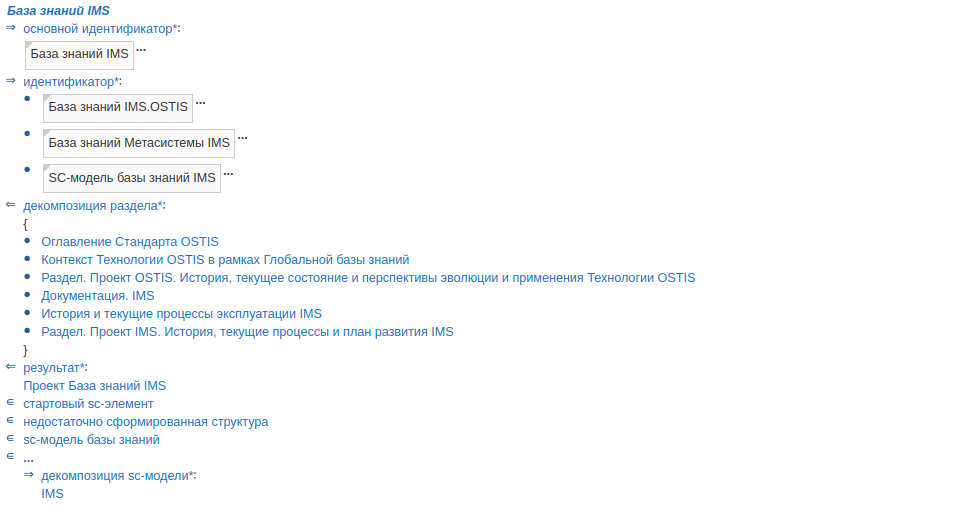
\includegraphics[scale=0.8, width=1.0\textwidth]{images/part7/chapter_ims_standard/ims_main_page.png}
	\caption{Cтартовая страница базы знаний Метасистемы OSTIS}
	\label{fig:main_page}
\end{figure}

Предлагаемое представление \textit{Стандарта OSTIS} обеспечивает эффективную семантическую навигацию по содержанию \textit{Стандарта OSTIS}, поскольку перейдя к соответствующему разделу \textit{Метасистемы OSTIS}, как представлено на рисунке \textit{\nameref{fig:table_of_contents}}, можно увидеть текущее оглавление \textit{Стандарта OSTIS}. 

\begin{figure}[H]
	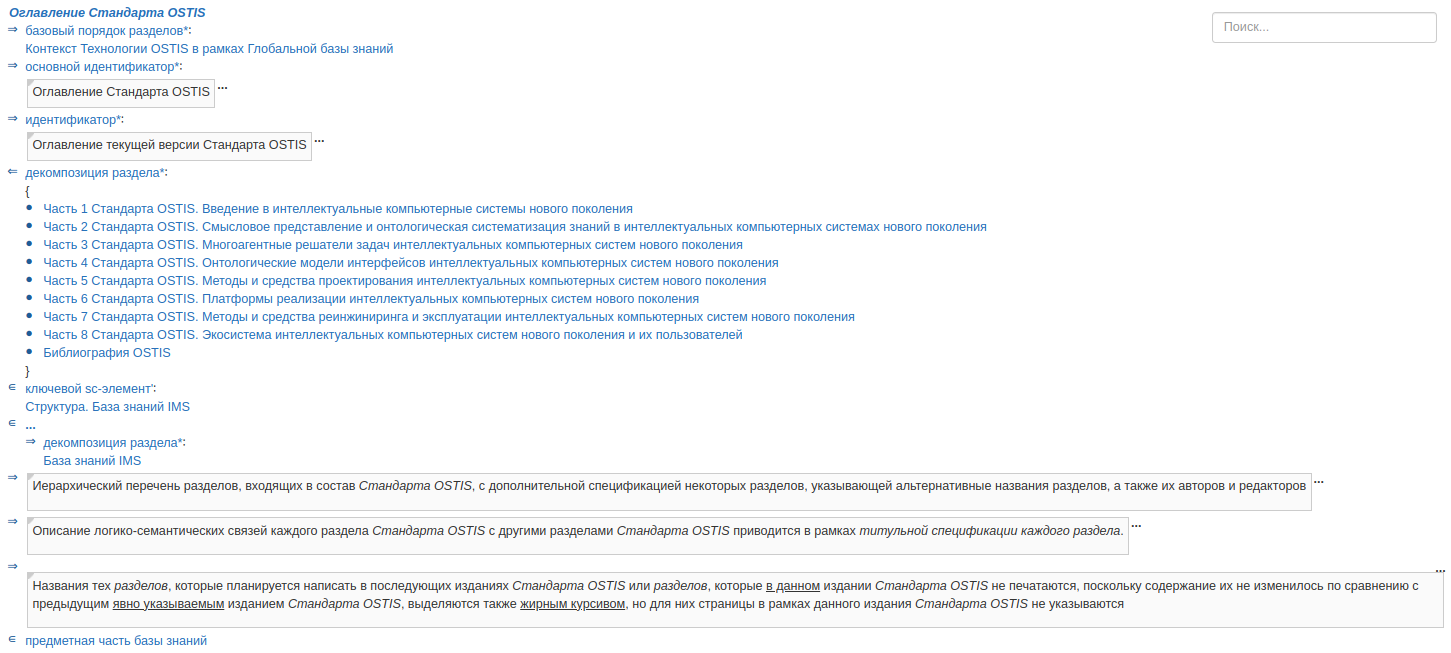
\includegraphics[scale=0.8, width=1.0\textwidth]{images/part7/chapter_ims_standard/table_of_contents.png}
	\caption{Оглавление Стандарта OSTIS}
	\label{fig:table_of_contents}
\end{figure}

Пользователю предоставляется возможность перейти к любой интересующей его теме, как показано на рисунке \textit{\nameref{fig:navigation}} и задавать \textit{Метасистеме OSTIS} широкий спектр нетривиальных вопросов о самых различных деталях и тонкостях \textit{Технологии OSTIS}, как представлено на рисунке \textit{\nameref{fig:question}} и получать ответы на заданные вопросы, как представлено на рисунке \textit{\nameref{fig:response}}. 

\begin{figure}[H]
	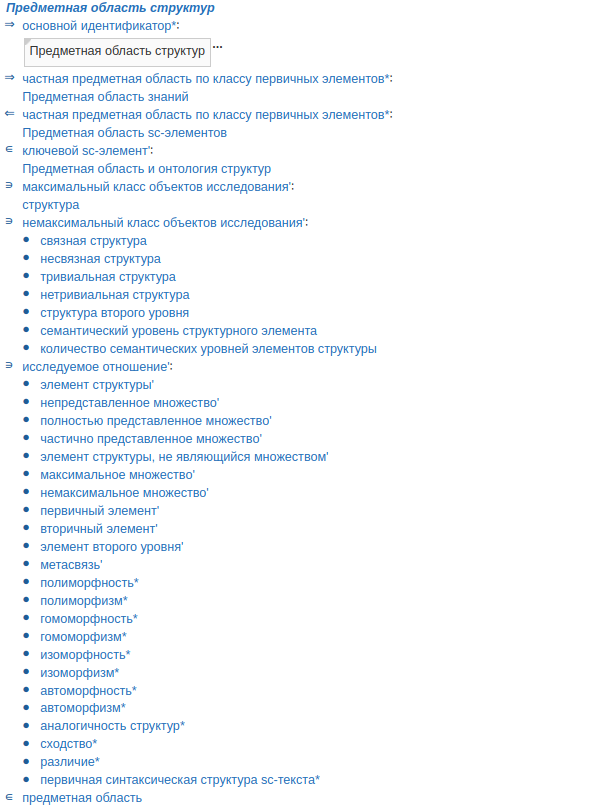
\includegraphics[scale=0.8, width=1.0\textwidth]{images/part7/chapter_ims_standard/navigation.png}
	\caption{Навигация по Оглавлению Стандарта OSTIS}
	\label{fig:navigation}
\end{figure}

\begin{figure}[H]
	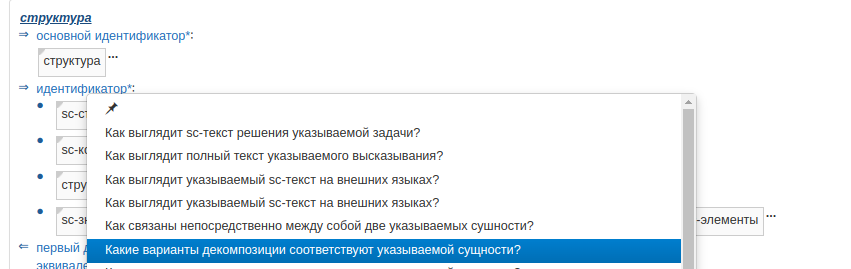
\includegraphics[scale=0.8, width=1.0\textwidth]{images/part7/chapter_ims_standard/question.png}
	\caption{Функция вопросов Метасистемы OSTIS}
	\label{fig:question}
\end{figure}

\begin{figure}[H]
	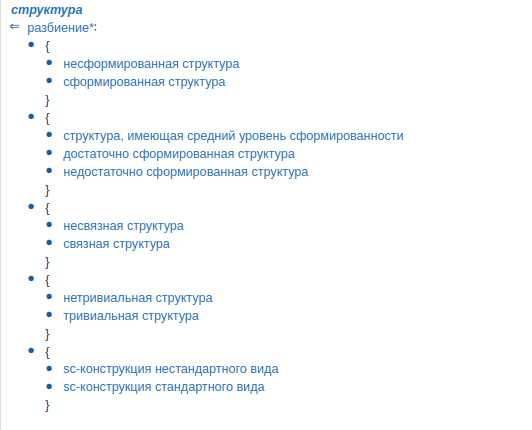
\includegraphics[scale=0.8, width=1.0\textwidth]{images/part7/chapter_ims_standard/response.png}
	\caption{Функция ответов Метасистемы OSTIS}
	\label{fig:response}
\end{figure}

По умолчанию ответы системы пользователю отображаются в SCn-коде, который является гипертекстовым вариантом внешнего отображения текстов SC-кода и может читаться как линейный текст.

\section*{Заключение к Главе~\ref{chapter_ims_standard}}

Для реализации кооперативного целенаправленного и адаптивного взаимодействия интеллектуальных компьютерных систем в рамках автоматически формируемых коллективов интеллектуальных компьютерных систем необходима семантическая совместимость интеллектуальных компьютерных систем, а это, в свою очередь, требует унификации интеллектуальных компьютерных систем. Унификация интеллектуальной компьютерной системы возможна только на основе общей формальной теории интеллектуальных компьютерных систем и соответствующего ей \textbf{стандарта интеллектуальных компьютерных систем}, а для этого необходима глубокая конвергенция различных направлений исследований в области искусственного интеллекта.

Поскольку результатом развития искусственного интеллекта как научной дисциплины является перманентная эволюция общей теории интеллектуальных компьютерных систем и соответствующего стандарта интеллектуальных компьютерных систем, для повышения темпов развития искусственного интеллекта и, соответственно, технологии разработки интеллектуальных компьютерных систем необходимо создание портала научно-технических знаний по искусственному интеллекту, обеспечивающего координацию деятельности специалистов, а также согласование и интеграцию результатов этой деятельности.

В главе рассмотрен подход к автоматизации процессов создания, развития и применения стандартов на основе Технологии OSTIS. На основе \textit{Стандарта Технологии OSTIS} рассмотрены основные принципы, лежащие в основе предлагаемого подхода к стандартизации.

Предложенный в данной главе подход позволяет обеспечить не только возможность автоматизации процессов создания, согласования и развития стандартов, но и позволяет значительно повысить эффективность процессов применения стандарта, как в ручном, так и в автоматическом режиме.

%%%%%%%%%%%%%%%%%%%%%%%%% referenc.tex %%%%%%%%%%%%%%%%%%%%%%%%%%%%%%
% sample references
% %
% Use this file as a template for your own input.
%
%%%%%%%%%%%%%%%%%%%%%%%% Springer-Verlag %%%%%%%%%%%%%%%%%%%%%%%%%%
%
% BibTeX users please use
% \bibliographystyle{}
% \bibliography{}
%
\biblstarthook{In view of the parallel print and (chapter-wise) online publication of your book at \url{www.springerlink.com} it has been decided that -- as a genreral rule --  references should be sorted chapter-wise and placed at the end of the individual chapters. However, upon agreement with your contact at Springer you may list your references in a single seperate chapter at the end of your book. Deactivate the class option \texttt{sectrefs} and the \texttt{thebibliography} environment will be put out as a chapter of its own.\\\indent
References may be \textit{cited} in the text either by number (preferred) or by author/year.\footnote{Make sure that all references from the list are cited in the text. Those not cited should be moved to a separate \textit{Further Reading} section or chapter.} If the citatiion in the text is numbered, the reference list should be arranged in ascending order. If the citation in the text is author/year, the reference list should be \textit{sorted} alphabetically and if there are several works by the same author, the following order should be used:
\begin{enumerate}
\item all works by the author alone, ordered chronologically by year of publication
\item all works by the author with a coauthor, ordered alphabetically by coauthor
\item all works by the author with several coauthors, ordered chronologically by year of publication.
\end{enumerate}
The \textit{styling} of references\footnote{Always use the standard abbreviation of a journal's name according to the ISSN \textit{List of Title Word Abbreviations}, see \url{http://www.issn.org/en/node/344}} depends on the subject of your book:
\begin{itemize}
\item The \textit{two} recommended styles for references in books on \textit{mathematical, physical, statistical and computer sciences} are depicted in ~\cite{science-contrib, science-online, science-mono, science-journal, science-DOI} and ~\cite{phys-online, phys-mono, phys-journal, phys-DOI, phys-contrib}.
\item Examples of the most commonly used reference style in books on \textit{Psychology, Social Sciences} are~\cite{psysoc-mono, psysoc-online,psysoc-journal, psysoc-contrib, psysoc-DOI}.
\item Examples for references in books on \textit{Humanities, Linguistics, Philosophy} are~\cite{humlinphil-journal, humlinphil-contrib, humlinphil-mono, humlinphil-online, humlinphil-DOI}.
\item Examples of the basic Springer style used in publications on a wide range of subjects such as \textit{Computer Science, Economics, Engineering, Geosciences, Life Sciences, Medicine, Biomedicine} are ~\cite{basic-contrib, basic-online, basic-journal, basic-DOI, basic-mono}. 
\end{itemize}
}

\begin{thebibliography}{99.}%
% and use \bibitem to create references.
%
% Use the following syntax and markup for your references if 
% the subject of your book is from the field 
% "Mathematics, Physics, Statistics, Computer Science"
%
% Contribution 
\bibitem{science-contrib} Broy, M.: Software engineering --- from auxiliary to key technologies. In: Broy, M., Dener, E. (eds.) Software Pioneers, pp. 10-13. Springer, Heidelberg (2002)
%
% Online Document
\bibitem{science-online} Dod, J.: Effective substances. In: The Dictionary of Substances and Their Effects. Royal Society of Chemistry (1999) Available via DIALOG. \\
\url{http://www.rsc.org/dose/title of subordinate document. Cited 15 Jan 1999}
%
% Monograph
\bibitem{science-mono} Geddes, K.O., Czapor, S.R., Labahn, G.: Algorithms for Computer Algebra. Kluwer, Boston (1992) 
%
% Journal article
\bibitem{science-journal} Hamburger, C.: Quasimonotonicity, regularity and duality for nonlinear systems of partial differential equations. Ann. Mat. Pura. Appl. \textbf{169}, 321--354 (1995)
%
% Journal article by DOI
\bibitem{science-DOI} Slifka, M.K., Whitton, J.L.: Clinical implications of dysregulated cytokine production. J. Mol. Med. (2000) doi: 10.1007/s001090000086 
%
\bigskip

% Use the following (APS) syntax and markup for your references if 
% the subject of your book is from the field 
% "Mathematics, Physics, Statistics, Computer Science"
%
% Online Document
\bibitem{phys-online} J. Dod, in \textit{The Dictionary of Substances and Their Effects}, Royal Society of Chemistry. (Available via DIALOG, 1999), 
\url{http://www.rsc.org/dose/title of subordinate document. Cited 15 Jan 1999}
%
% Monograph
\bibitem{phys-mono} H. Ibach, H. L\"uth, \textit{Solid-State Physics}, 2nd edn. (Springer, New York, 1996), pp. 45-56 
%
% Journal article
\bibitem{phys-journal} S. Preuss, A. Demchuk Jr., M. Stuke, Appl. Phys. A \textbf{61}
%
% Journal article by DOI
\bibitem{phys-DOI} M.K. Slifka, J.L. Whitton, J. Mol. Med., doi: 10.1007/s001090000086
%
% Contribution 
\bibitem{phys-contrib} S.E. Smith, in \textit{Neuromuscular Junction}, ed. by E. Zaimis. Handbook of Experimental Pharmacology, vol 42 (Springer, Heidelberg, 1976), p. 593
%
\bigskip
%
% Use the following syntax and markup for your references if 
% the subject of your book is from the field 
% "Psychology, Social Sciences"
%
%
% Monograph
\bibitem{psysoc-mono} Calfee, R.~C., \& Valencia, R.~R. (1991). \textit{APA guide to preparing manuscripts for journal publication.} Washington, DC: American Psychological Association.
%
% Online Document
\bibitem{psysoc-online} Dod, J. (1999). Effective substances. In: The dictionary of substances and their effects. Royal Society of Chemistry. Available via DIALOG. \\
\url{http://www.rsc.org/dose/Effective substances.} Cited 15 Jan 1999.
%
% Journal article
\bibitem{psysoc-journal} Harris, M., Karper, E., Stacks, G., Hoffman, D., DeNiro, R., Cruz, P., et al. (2001). Writing labs and the Hollywood connection. \textit{J Film} Writing, 44(3), 213--245.
%
% Contribution 
\bibitem{psysoc-contrib} O'Neil, J.~M., \& Egan, J. (1992). Men's and women's gender role journeys: Metaphor for healing, transition, and transformation. In B.~R. Wainrig (Ed.), \textit{Gender issues across the life cycle} (pp. 107--123). New York: Springer.
%
% Journal article by DOI
\bibitem{psysoc-DOI}Kreger, M., Brindis, C.D., Manuel, D.M., Sassoubre, L. (2007). Lessons learned in systems change initiatives: benchmarks and indicators. \textit{American Journal of Community Psychology}, doi: 10.1007/s10464-007-9108-14.
%
%
% Use the following syntax and markup for your references if 
% the subject of your book is from the field 
% "Humanities, Linguistics, Philosophy"
%
\bigskip
%
% Journal article
\bibitem{humlinphil-journal} Alber John, Daniel C. O'Connell, and Sabine Kowal. 2002. Personal perspective in TV interviews. \textit{Pragmatics} 12:257--271
%
% Contribution 
\bibitem{humlinphil-contrib} Cameron, Deborah. 1997. Theoretical debates in feminist linguistics: Questions of sex and gender. In \textit{Gender and discourse}, ed. Ruth Wodak, 99--119. London: Sage Publications.
%
% Monograph
\bibitem{humlinphil-mono} Cameron, Deborah. 1985. \textit{Feminism and linguistic theory.} New York: St. Martin's Press.
%
% Online Document
\bibitem{humlinphil-online} Dod, Jake. 1999. Effective substances. In: The dictionary of substances and their effects. Royal Society of Chemistry. Available via DIALOG. \\
http://www.rsc.org/dose/title of subordinate document. Cited 15 Jan 1999
%
% Journal article by DOI
\bibitem{humlinphil-DOI} Suleiman, Camelia, Daniel C. O'Connell, and Sabine Kowal. 2002. `If you and I, if we, in this later day, lose that sacred fire...': Perspective in political interviews. \textit{Journal of Psycholinguistic Research}. doi: 10.1023/A:1015592129296.
%
%
%
\bigskip
%
%
% Use the following syntax and markup for your references if 
% the subject of your book is from the field 
% "Computer Science, Economics, Engineering, Geosciences, Life Sciences"
%
%
% Contribution 
\bibitem{basic-contrib} Brown B, Aaron M (2001) The politics of nature. In: Smith J (ed) The rise of modern genomics, 3rd edn. Wiley, New York 
%
% Online Document
\bibitem{basic-online} Dod J (1999) Effective Substances. In: The dictionary of substances and their effects. Royal Society of Chemistry. Available via DIALOG. \\
\url{http://www.rsc.org/dose/title of subordinate document. Cited 15 Jan 1999}
%
% Journal article by DOI
\bibitem{basic-DOI} Slifka MK, Whitton JL (2000) Clinical implications of dysregulated cytokine production. J Mol Med, doi: 10.1007/s001090000086
%
% Journal article
\bibitem{basic-journal} Smith J, Jones M Jr, Houghton L et al (1999) Future of health insurance. N Engl J Med 965:325--329
%
% Monograph
\bibitem{basic-mono} South J, Blass B (2001) The future of modern genomics. Blackwell, London 
%
\end{thebibliography}

